\documentclass[10pt]{article}
\usepackage[margin=2cm]{geometry}
\usepackage{amsmath,amssymb}
\usepackage{booktabs}
\usepackage{graphicx}
\usepackage{float}
\usepackage[font=small,labelfont=bf]{caption}
\usepackage[compact]{titlesec}
\usepackage{enumitem}
\usepackage{microtype}
\usepackage[hidelinks]{hyperref}
\setlist{itemsep=1pt,topsep=3pt}
\setlength{\parskip}{4pt}
\setlength{\parindent}{0pt}
\graphicspath{{figures/}}
\newcommand{\fig}[1]{Figure~\ref{#1}}
\newcommand{\tab}[1]{Table~\ref{#1}}

\begin{document}
\sloppy

\begin{center}
{\LARGE SuperMimic on Kangaroo, M4: the online loop on \texttt{dev}}\\[4pt]
Twelve hours of SuperMimic from scratch on the local GPU, against the PPO-Sim baseline. Branch
\texttt{omm/supermimic} of pal\_mjlab, 24 October 2026.
\end{center}

\section*{Summary}

M4 ran SuperMimic's full online loop for the first time: Algorithm~A.1 from scratch on the 2.5\,h
\texttt{dev} motion set. The environment and the 12\,h local-GPU budget are the same as the PPO-Sim
baseline's.

\begin{itemize}
  \item \textbf{At its peaks SuperMimic beats PPO-Sim, about twice as fast.}
  \begin{itemize}
    \item It matched PPO-Sim's 12\,h tracking return after \textbf{5.7\,h}.
    \item Its best checkpoint fails \textbf{3} of 1296 clips (PPO-Sim: 25), with tracking return
    \textbf{0.832} (PPO-Sim: 0.742).
    \item Its errors are 22--32\% lower on legs, arms and torso.
    \item It used 6$\times$ fewer simulator steps.
  \end{itemize}
  \item \textbf{But training oscillates.} Every 1.3--2\,h the policy collapses from strong to failing
  most clips, then recovers to a higher peak. Four of the 15 checkpoints after 5.7\,h sit in a
  collapse, including the last one.
  \item \textbf{The critic drives each collapse.} Its value jumps 3--5$\times$ while the simulator's
  reward is still normal. The policy then follows the critic instead of the reward, and the simulator
  collapses.
  \item \textbf{The world model and the learned failure head work online.} Imagination tracks the
  simulator within a few percent, and once refit online the head detects failures as well as the env's
  rule (AUC 0.999).
\end{itemize}

\textbf{Next.} The paper's exact settings on the cluster (TF32, replay 1000), to test whether our two
memory-forced deviations cause the oscillation. Then the critic loop if they don't. Meanwhile, keep the
best checkpoint, not the last.


\section{The run}

\textbf{What ran.} Algorithm~A.1 from scratch, on the task with the same environment and gains as
PPO-Sim, \texttt{Mjlab-SuperMimic-Flat-Pal-Kangaroo-Grippers-ArmWaist1Hz}. It was launched with
mjlab's \texttt{train} CLI through the resumable wrapper. Each iteration:
\begin{enumerate}
  \item collects about 2.5 simulator steps from 4096 envs, with action noise $\mathcal N(0, 0.1^2)$;
  \item fits the world model on 10 batches of 2048 windows ($k = 8$);
  \item takes one BPTT step through 4096 imagined rollouts of 32 steps, with the learned failure head
  (D31) and the critic;
  \item fits the critic on the rollouts' $\lambda$-returns (5 epochs of 4 minibatches).
\end{enumerate}
Everything follows Table~A.5 except two settings forced by the 16\,GB GPU (D16): bf16 learning updates
instead of TF32, and a replay of 500 instead of 1000 steps per env.

\textbf{Budget.} 12\,h on the RTX 5060 Ti, the same budget as the PPO-Sim baseline, with no
interruption.
\begin{itemize}
  \item 27,510 iterations, 1.57\,s each (collect 0.15\,s, world model 0.31\,s, policy and critic
  1.11\,s), at 11.3\,GB.
  \item About 0.28 billion simulator steps; PPO-Sim used 1.7 billion in its 12\,h.
\end{itemize}

\textbf{How it is compared.} Checkpoints every 1000 iterations (about 26\,min) were benchmarked the
paper's way (\texttt{eval.py}): every \texttt{dev} clip once from its first frame, with no
randomization or noise. PPO-Sim's checkpoints were benchmarked the same way. Runs are compared at
equal training hours, since an ``iteration'' means very different amounts of work in the two
methods.

\section{Benchmark: SuperMimic vs PPO-Sim}

\begin{figure}[H]
\centering
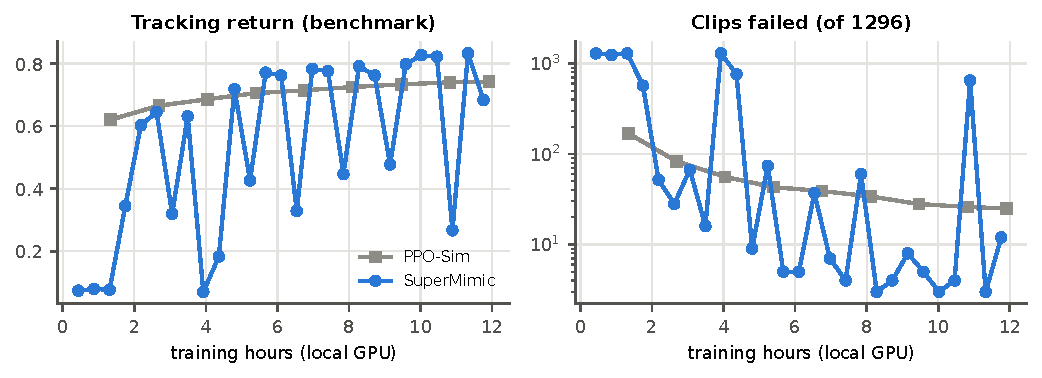
\includegraphics[width=\textwidth]{benchmark.pdf}
\caption{The paper's benchmark (every \texttt{dev} clip once from its first frame) of each checkpoint
vs training hours on the local GPU. PPO-Sim: every 1000 PPO iterations; SuperMimic: every 1000
SuperMimic iterations (about 26\,min).}
\label{fig:benchmark}
\end{figure}

\begin{table}[H]
\centering\small
\caption{Key checkpoints. Errors are root-relative body-position errors, averaged over each clip. All
checkpoints are listed in the appendix.}
\label{tab:summary}
\setlength{\tabcolsep}{4pt}
\resizebox{\textwidth}{!}{\begin{tabular}{lrrrrrrr}\toprule
policy & hours & iteration & failed & tracking return & legs [cm] & arms [cm] & torso [cm] \\\midrule
PPO-Sim, final & 11.9 & 8,800 & 25 & 0.742 & 6.4 & 10.8 & 2.4 \\
SuperMimic, first checkpoint above it & 5.7 & 13,000 & 5 & 0.771 & 6.3 & 9.4 & 2.0 \\
SuperMimic, best checkpoint & 11.3 & 26,000 & 3 & 0.832 & 5.0 & 7.3 & 1.7 \\
SuperMimic, last checkpoint & 11.8 & 27,000 & 12 & 0.684 & 7.7 & 14.5 & 2.5 \\
\bottomrule\end{tabular}
}
\end{table}

\begin{itemize}
  \item \textbf{Faster to PPO-Sim's level.} SuperMimic first exceeds PPO-Sim's final tracking return
  (0.742) at 5.7\,h, with 5 failures instead of 25. PPO-Sim reaches 0.742 only at the end of its
  12\,h.
  \item \textbf{Better at its best.} The best checkpoint (11.3\,h) fails 3 clips. Its errors are
  5.0\,cm on legs (PPO-Sim: 6.4), 7.3\,cm on arms (10.8) and 1.7\,cm on torso (2.4), and its tracking
  return is 0.832.
  \item \textbf{Not reliably.} 10 of the 15 checkpoints from 5.7\,h on beat PPO-Sim's final policy.
  Four are in a collapse, with tracking return 0.27--0.48 and up to 650 failures. The last checkpoint
  (0.684) is on the way down from a peak. The peaks rise steadily (0.645, 0.771, 0.791, 0.826, 0.832),
  so learning itself progresses.
  \item \textbf{With much less simulator data.} About 0.28 billion simulator steps against PPO-Sim's
  1.7 billion. Most of the learning happens in imagination: each iteration differentiates through
  $4096 \times 32$ imagined steps.
\end{itemize}

The two runs also log the same training-time signals (\fig{fig:vsppo}). They are measured on the
training starts, with exploration, so they are less clean than the benchmark, but they show the same
picture at a finer time resolution. From about 5\,h on, SuperMimic's sampler return is mostly above
PPO-Sim's. Its tracking errors spike with every collapse, and between collapses approach PPO-Sim's.

\begin{figure}[H]
\centering
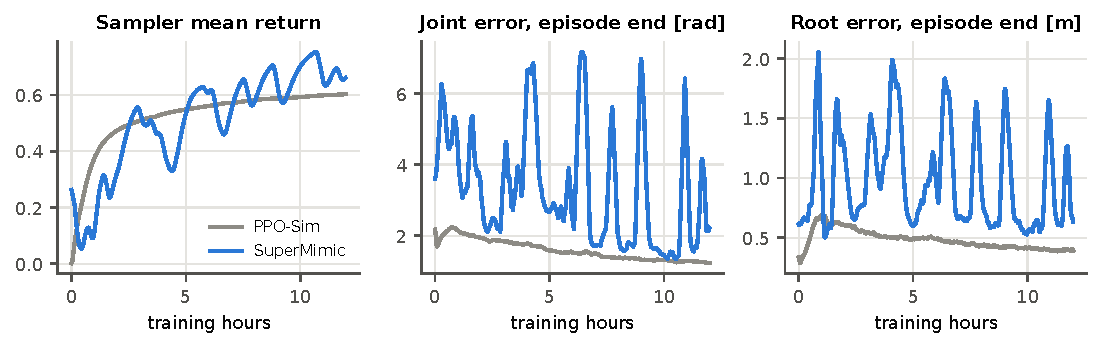
\includegraphics[width=\textwidth]{vs_ppo_training.pdf}
\caption{Signals both runs log during training (moving averages): the return-based sampler's mean
normalized return, and the joint and root errors when episodes end.}
\label{fig:vsppo}
\end{figure}

\section{What happens during training}

\begin{figure}[H]
\centering
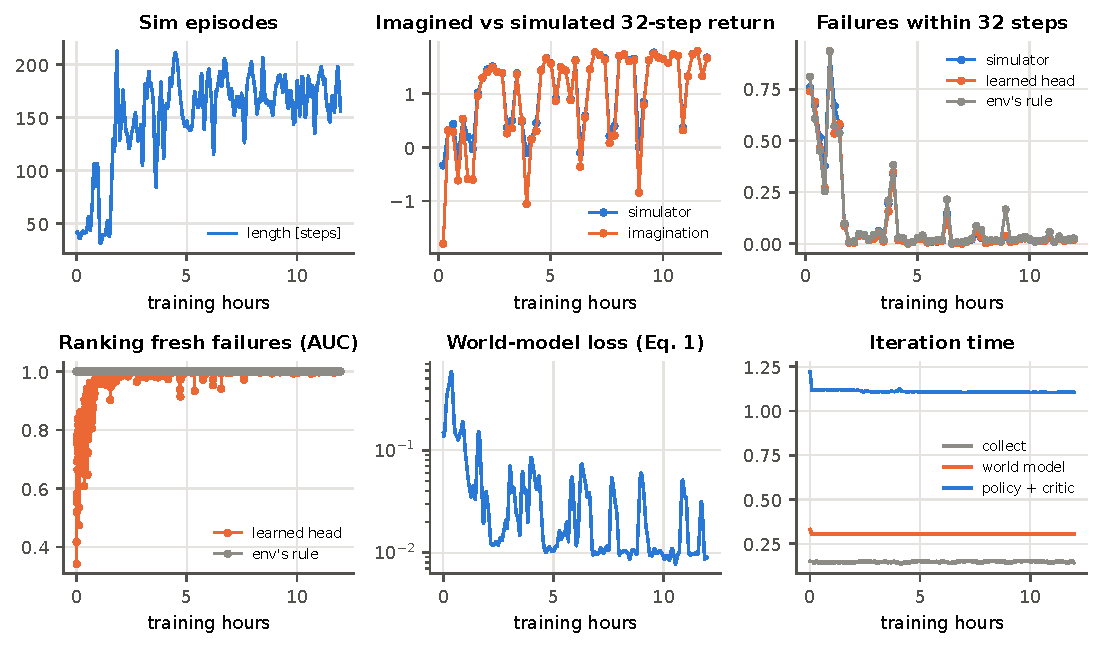
\includegraphics[width=\textwidth]{training.pdf}
\caption{SuperMimic's own signals. Top: simulator episode length; imagined vs simulated 32-step return
of the current policy from the same states (every 500 iterations); failures within those 32 steps,
simulated and predicted. Bottom: how the learned head and the env's rule rank fresh simulator failures;
world-model loss; time per iteration.}
\label{fig:training}
\end{figure}

\textbf{The world model keeps up with the policy} (\fig{fig:training}).
\begin{itemize}
  \item \textbf{Imagination matches the simulator.} The imagined and simulated 32-step returns agree
  within a few percent (correlation 0.97--1.0), including at most dips. They diverge briefly while a
  collapse is under way.
  \item \textbf{Its loss follows the policy.} The world-model loss settles at about 0.01 and spikes
  whenever the policy shifts, then returns: the model is refit on the new states, as Alg.~A.1 intends.
  \item \textbf{The learned failure head matches the rule after about 1.5\,h} (AUC 0.999--1.0 on fresh
  failures), and its predicted failure rate tracks the simulator's. In M3 the frozen head missed the
  new policy's falls; refitting online fixes that, as hoped when choosing it (D31).
\end{itemize}

\begin{figure}[H]
\centering
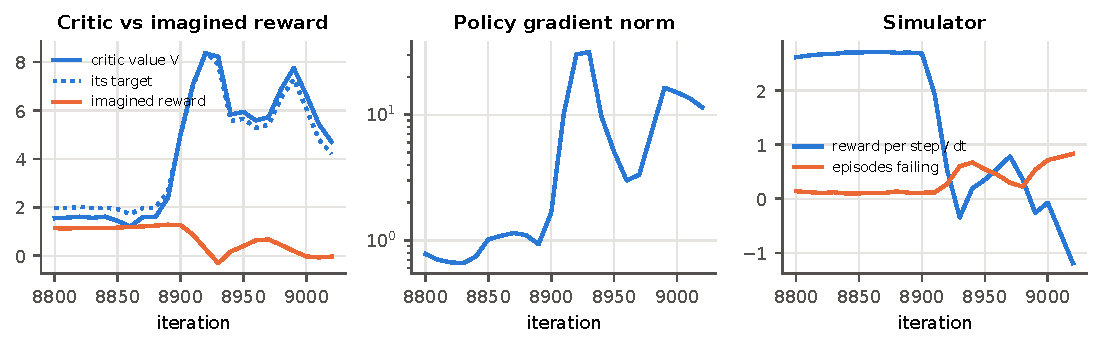
\includegraphics[width=\textwidth]{collapse.pdf}
\caption{One collapse at full resolution (iterations 8800--9020; the benchmark had 16 failures at 8000
and 1296 at 9000). Left: critic value of the start states, its $\lambda$-return target, and the
imagined 32-step reward. Middle: norm of the policy gradient, before clipping. Right: the simulator's
reward per step and the share of episodes ending in a failure.}
\label{fig:collapse}
\end{figure}

\textbf{The critic drives each collapse} (\fig{fig:collapse}). Each collapse follows the same
sequence:
\begin{enumerate}
  \item \textbf{The critic's value jumps first,} from about 1.6 to 8.4 within 40 iterations. Meanwhile
  the simulator's reward and failure rate are unchanged. The $\lambda$-return targets follow the
  value, because they bootstrap on it (Eq.~3).
  \item \textbf{The policy follows the critic.} The policy gradient grows from about 1 to 30 and the
  imagined reward over the 32 steps drops. The update trades real reward for critic value at step 32.
  \item \textbf{The simulator collapses.} Reward per step falls to about zero and the share of episodes
  ending in a failure goes from 11\% to 67\%.
  \item \textbf{Recovery} begins once the critic has been refit on rollouts of the collapsed policy;
  its values come down and the policy relearns.
\end{enumerate}
This is a critic overestimation loop: a deterministic actor maximizing a bootstrapped critic that has
no target network. It is the same failure mode M3 showed on the frozen model, here recovering because
everything is refit online. The paper reports very stable training with the same no-target-network
design, so something in our setup makes the loop easier to trigger.

\textbf{Our deviations from the paper,} the first suspects:
\begin{itemize}
  \item \textbf{bf16 learning updates} (D16). The critic's $\lambda$-return targets and the value at
  step 32 are computed in bf16 inside imagination, as is the whole policy gradient.
  \item \textbf{Replay of 500 instead of 1000 steps per env} (D16). The world model and the start
  states cover a shorter history.
  \item \textbf{Our own choices where the paper is silent:}
  \begin{itemize}
    \item privileged critic inputs (root-pose error, time left in the clip; D7);
    \item critic input normalization from the simulator's observations (D34).
  \end{itemize}
  \item \textbf{The robot.} Kangaroo has heavier, softer arms and a closed-chain leg, unlike the
  paper's G1.
\end{itemize}

\section{Gate and next steps}

\textbf{Gate.}
\begin{itemize}
  \item ``$\geq$ PPO-Sim on \texttt{dev}'': met at the peaks, about $2\times$ faster to PPO-Sim's
  12\,h level and better at the best checkpoint.
  \item Not met for training stability.
  \item The critic vs no-critic comparison is still to run.
\end{itemize}

\textbf{Next steps,} in order:
\begin{enumerate}
  \item \textbf{Run the paper's exact settings on the cluster} (\texttt{dev}, TF32, replay 1000). This
  removes both memory-forced deviations at once. If it is stable, the oscillation came from them; then
  scale to \texttt{full} (250.9\,h). Commands are in \texttt{docs/supermimic/README.md}.
  \item \textbf{If it still oscillates, investigate the critic loop,} one change at a time, each judged
  on the benchmark:
  \begin{itemize}
    \item policy learning rate (M3 showed strong sensitivity);
    \item critic inputs without the privileged terms;
    \item frozen critic input normalization.
  \end{itemize}
  \item \textbf{Select checkpoints by benchmark.} With collapses, the last checkpoint is often not the
  best (here 0.684 vs 0.832). Keep benchmarking checkpoints during training.
  \item \textbf{Then the remaining ablations and M5:} the critic ablation (paper Fig.~4b), $H = 16$ if
  needed, \texttt{full} on the cluster, and the data-scaling comparison with PPO-Sim (paper
  Fig.~3).
\end{enumerate}

\appendix
\section{All checkpoints}

\begin{table}[H]
\centering\small
\caption{The paper's benchmark of every checkpoint of both runs (1296 \texttt{dev} clips).}
\label{tab:benchmark}
\begin{tabular}{lrrrrrrr}\toprule
run & iteration & hours & failed & tracking return & legs [cm] & arms [cm] & torso [cm] \\\midrule
PPO-Sim & 1,000 & 1.3 & 169 & 0.620 & 8.5 & 15.2 & 3.4 \\
PPO-Sim & 2,000 & 2.7 & 83 & 0.665 & 7.8 & 13.9 & 3.2 \\
PPO-Sim & 3,000 & 4.0 & 56 & 0.686 & 7.4 & 13.5 & 2.8 \\
PPO-Sim & 4,000 & 5.4 & 43 & 0.705 & 7.1 & 12.5 & 2.9 \\
PPO-Sim & 5,000 & 6.7 & 39 & 0.714 & 6.9 & 12.2 & 2.7 \\
PPO-Sim & 6,000 & 8.1 & 34 & 0.725 & 6.7 & 11.7 & 2.5 \\
PPO-Sim & 7,000 & 9.5 & 28 & 0.733 & 6.7 & 11.3 & 2.6 \\
PPO-Sim & 8,000 & 10.8 & 26 & 0.740 & 6.5 & 11.0 & 2.4 \\
PPO-Sim & 8,800 & 11.9 & 25 & 0.742 & 6.4 & 10.8 & 2.4 \\
\midrule
SuperMimic & 1,000 & 0.4 & 1295 & 0.074 & 17.3 & 29.2 & 9.2 \\
SuperMimic & 2,000 & 0.9 & 1244 & 0.079 & 22.5 & 38.0 & 7.5 \\
SuperMimic & 3,000 & 1.3 & 1295 & 0.077 & 22.7 & 35.2 & 7.2 \\
SuperMimic & 4,000 & 1.7 & 570 & 0.344 & 13.8 & 28.2 & 6.1 \\
SuperMimic & 5,000 & 2.2 & 52 & 0.602 & 10.1 & 19.5 & 3.8 \\
SuperMimic & 6,000 & 2.6 & 28 & 0.645 & 7.9 & 16.5 & 3.3 \\
SuperMimic & 7,000 & 3.1 & 67 & 0.320 & 13.9 & 38.4 & 5.6 \\
SuperMimic & 8,000 & 3.5 & 16 & 0.631 & 7.9 & 16.1 & 2.7 \\
SuperMimic & 9,000 & 3.9 & 1296 & 0.070 & 21.8 & 40.8 & 7.3 \\
SuperMimic & 10,000 & 4.4 & 760 & 0.183 & 17.2 & 44.7 & 6.4 \\
SuperMimic & 11,000 & 4.8 & 9 & 0.718 & 7.0 & 12.6 & 2.7 \\
SuperMimic & 12,000 & 5.2 & 74 & 0.426 & 15.1 & 24.9 & 3.6 \\
SuperMimic & 13,000 & 5.7 & 5 & 0.771 & 6.3 & 9.4 & 2.0 \\
SuperMimic & 14,000 & 6.1 & 5 & 0.762 & 6.1 & 9.9 & 1.9 \\
SuperMimic & 15,000 & 6.5 & 37 & 0.329 & 13.5 & 39.0 & 3.7 \\
SuperMimic & 16,000 & 7.0 & 7 & 0.783 & 5.9 & 9.4 & 2.1 \\
SuperMimic & 17,000 & 7.4 & 4 & 0.776 & 5.6 & 9.7 & 1.9 \\
SuperMimic & 18,000 & 7.8 & 60 & 0.446 & 13.3 & 28.6 & 5.7 \\
SuperMimic & 19,000 & 8.3 & 3 & 0.791 & 5.5 & 9.3 & 1.8 \\
SuperMimic & 20,000 & 8.7 & 4 & 0.762 & 6.1 & 9.8 & 1.9 \\
SuperMimic & 21,000 & 9.2 & 8 & 0.477 & 13.2 & 27.8 & 3.7 \\
SuperMimic & 22,000 & 9.6 & 5 & 0.798 & 6.3 & 8.2 & 1.9 \\
SuperMimic & 23,000 & 10.0 & 3 & 0.826 & 5.5 & 7.3 & 1.7 \\
SuperMimic & 24,000 & 10.5 & 4 & 0.822 & 5.2 & 7.7 & 1.8 \\
SuperMimic & 25,000 & 10.9 & 650 & 0.267 & 16.7 & 43.6 & 4.9 \\
SuperMimic & 26,000 & 11.3 & 3 & 0.832 & 5.0 & 7.3 & 1.7 \\
SuperMimic & 27,000 & 11.8 & 12 & 0.684 & 7.7 & 14.5 & 2.5 \\
\bottomrule\end{tabular}

\end{table}

\section{Reproduction}

\begin{footnotesize}
\begin{verbatim}
# training (12 h local GPU, bf16, replay 500), through the GPU queue
python -m pal_mjlab.scripts.supermimic.train Mjlab-SuperMimic-Flat-Pal-Kangaroo-Grippers-ArmWaist1Hz \
  --env.commands.motion.subset dev --agent.algorithm.precision bf16 --agent.replay-steps 500 \
  --agent.experiment-name supermimic_wm_1hz --agent.run-name dev-local --agent.save-interval 1000
# benchmark of the checkpoints
python -m pal_mjlab.scripts.supermimic.eval --task Mjlab-SuperMimic-Flat-Pal-Kangaroo-Grippers-ArmWaist1Hz \
  --checkpoints <run>/model_*.pt --out-dir logs/supermimic_eval/wm_1hz_dev_local
# figures, tables, this report
python docs/supermimic/m4/make_figures.py && (cd docs/supermimic/m4 && latexmk -pdf report.tex)
\end{verbatim}
\end{footnotesize}


\end{document}
